\documentclass[journal]{IEEEtran}
\usepackage{filecontents}
\usepackage{cite}

\usepackage{colortbl}




\makeatletter
\def\endthebibliography{%
	\def\@noitemerr{\@latex@warning{Empty `thebibliography' environment}}%
	\endlist
}
\makeatother

\usepackage{stfloats}


\usepackage{url}
\hyphenation{op-tical net-works semi-conduc-tor}    

\title{Algoritmos de reconocimiento automático de patrones en computador de placa reducida para la detección de fibrilación auricular}

\author{Autores \\ %\IEEEauthorblockN{some author afiliation}
\and
Autores
 \\ \IEEEauthorblockN{Servicio Nacional de Aprendizaje, Centro de Electriciad Electrónica y Telecomunicaciones}
}


\ifCLASSINFOpdf
\usepackage[pdftex]{graphicx}
%declare the path(s) where your graphic files are
%\graphicspath{{../pdf/}{../jpeg/}}
%and their extensions so you won't have to specify these with
%every instance of \includegraphics
%\DeclareGraphicsExtensions{.pdf,.jpeg,.png}
\else
%or other class option (dvipsone, dvipdf, if not using dvips). graphicx
%will default to the driver specified in the system graphics.cfg if no
%driver is specified.
\usepackage[dvips]{graphicx}
%declare the path(s) where your graphic files are
%\graphicspath{{../eps/}}
%and their extensions so you won't have to specify these with
%every instance of \includegraphics
%\DeclareGraphicsExtensions{.eps}
\fi
% graphicx was written by David Carlisle and Sebastian Rahtz. It is
% required if you want graphics, photos, etc. graphicx.sty is already
% installed on most LaTeX systems. The latest version and documentation
% can be obtained at: 
% http://www.ctan.org/pkg/graphicx
% Another good source of documentation is "Using Imported Graphics in
% LaTeX2e" by Keith Reckdahl which can be found at:
% http://www.ctan.org/pkg/epslatex
%
% latex, and pdflatex in dvi mode, support graphics in encapsulated
% postscript (.eps) format. pdflatex in pdf mode supports graphics
% in .pdf, .jpeg, .png and .mps (metapost) formats. Users should ensure
% that all non-photo figures use a vector format (.eps, .pdf, .mps) and
% not a bitmapped formats (.jpeg, .png). The IEEE frowns on bitmapped formats
% which can result in "jaggedy"/blurry rendering of lines and letters as
% well as large increases in file sizes.
%
% You can find documentation about the pdfTeX application at:
% http://www.tug.org/applications/pdftex
%


\usepackage[spanish]{babel}
\usepackage[utf8]{inputenc}


%\usepackage[backend=bibtex,style=ieee-alphabetic,natbib=true]{biblatex} %added
\usepackage[numbers]{natbib}
% \usepackage[authoryear,round,longnamesfirst]{natbib}

\begin{document}
\title{Medición de saturación de oxígeno usando aplicación de telemetría}
\maketitle


\begin{abstract}


%El desarrollo de dispositivos portables, que permita la detección en tiempo real de fibrilación auricular, requiere la implementación de algoritmos de reconocimiento automático de patrones con la metodología adecuada para su ejecución en sistemas embebidos. En el presente artículo se expone la implementación de una red neuronal artificial (ANN), una máquina de soporte vectorial (SVM) y un algoritmo de K vecinos más cercanos (KNN) en un computador de placa reducida para así comparar su desempeño en cuanto a la capacidad de detección de esta arritmia y el tiempo de respuesta asociado en su ejecución en tiempo real. La base de datos MIT-BIH AFIB es usada para el entrenamiento y validación de los algoritmos previa extracción de parámetros asociados a la transformada wavelet estacionaria. Se encontraron resultados entre el $90\%$ y $96\%$ para la sensibilidad y especificidad de los algoritmos mencionados y tiempos de respuesta variados entre $12 s$ y $16 s$. 

   
\end{abstract}
\IEEEpeerreviewmaketitle

\begin{IEEEkeywords}
	Saturación de oxígeno, MAX30102, pletismografía, embebido, densidad espectral de potencia, telemetría.
\end{IEEEkeywords}


\section{Introducción}

A

\IEEEPARstart{E}{p}idemología de enferedades respiratorias y cardiovasculares.

%\IEEEPARstart{L}{a} fibrilación auricular es una arritmia cardíaca que resulta ser la más frecuente en el ser humano. El 1\% de la población general y hasta 10\% de mayores de 80 años la padece \cite{uso_monitor_cardiaco}. De hecho, con el aumento de la expectativa de vida, esta arritmia se está convirtiendo en una de las enfermedades de mayor prevalencia \cite{clinica_monitoria_externa} \cite{wavelet_svm_afib} y con muy elevados gastos para los sistemas de salud (en países desarrollados se considera un gasto del 2.5\% de los gastos generales \cite{uso_monitor_cardiaco}).

Descripción de fisiología asociada a enfermedades cardiorespiratorias.
Importancia de medición de oxígeno en sangre y bondandes de telemedicina
Hay escasez de tecnologías disponibles con el alcance de monitorizacion telemétrica de oxígeno en sangre.

Descripción del oxímetro de pulso y dificultades para medir spo2

\begin{figure}[!h]
	\centering
	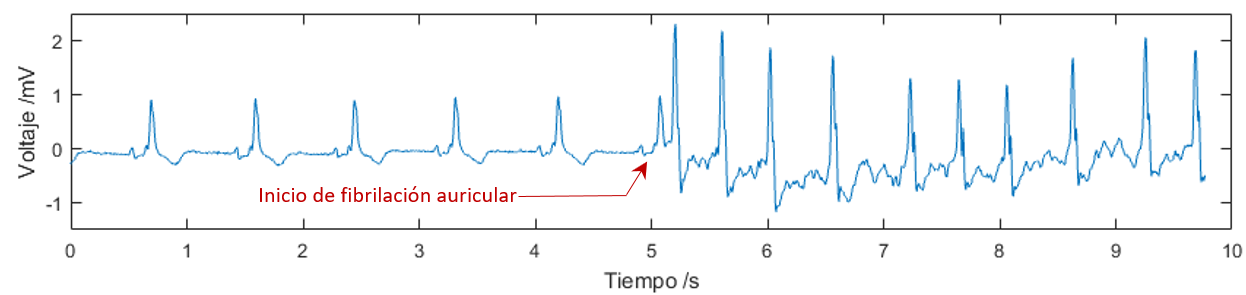
\includegraphics[width=3.5in]{mis_senales2.png}
	% where an .eps filename suffix will be assumed under latex, 
	% and a .pdf suffix will be assumed for pdflatex; or what has been declared
	% via \DeclareGraphicsExtensions.
	\caption{principio de funcionamiento oximetro de pulso \cite{physiobank} }.
	
	\label{imagen_ecg}
\end{figure}

Descripción de telemedicina y telemetría y dificultades en el desarrollo de monitor telemétrico.


El present artículo aborla la medicion de spo2 mediante tlemetria con la respectiva evaluación de resultados para aplicaciones futuras en telemedicina 



%En la fibrilación auricular, las aurículas son excitadas aleatoriamente y eventualmente se anula el impulso generado por el nodo sinoatrial (en la figura \ref{imagen_ecg} se presenta su trazado electrocardiográfico). Como consecuencia, el corazón presenta un progresivo déficit de bombeo de sangre, incrementando el riesgo de un infarto hasta cuatro veces  \cite{journal_afib}, de hecho "se calcula que el 15\% de los eventos cerebro-vasculares se atribuyen a esta arritmia, los cuales son más graves o discapacitantes que los no relacionados con ella" \cite{utilidad_monitor_externo} lo que aumenta la probabilidad de muerte o invalidez de la población afectada \cite{artificial_intelligence}. Para algunas personas la arritmia se presenta continuamente, y para otras, el ritmo normal puede suceder después de cierto tiempo (tiempos tan variados como arritmias de apenas un segundo a días) \cite{artificial_intelligence}. 




%De ahí que sus altos niveles de incidencia a nivel mundial generen un interés particular en el desarrollo de tecnologías para su diagnóstico \cite{uso_monitor_cardiaco}. Sin embargo, su  difícil detección en algunos casos, y la ocurrencia asintomática en otros,  son algunas de las problemáticas que enfrenta el desarrollo de tecnologías para su diagnóstico oportuno.

%Actualmente, en cuanto a las herramientas tecnológicas para el diagnóstico de esta arritmia se cuenta con equipos de electrocardiografía que si bien resultan ser la herramienta más asequible para el paciente, son insuficientes en el manejo clínico de pacientes con fibrilación auricular, dado el carácter asintomático y paroxístico de esta arritmia  \cite{monitores_externos} \cite{uso_monitor_cardiaco}. Por otra parte, el equipo Holter permite monitorizar al paciente por medio de 3 a 5 electrodos, durante un periodo de uno a dos días; terminado este tiempo, en el que el paciente sigue su rutina diaria normal, se transfieren los datos a un computador de escritorio y el especialista realiza el análisis manual de la información recogida. Esta monitorización ofrece una mayor sensibilidad de diagnóstico, del 15 al 28\% frente a la casi nula con el uso de electrocardiograma convencional \cite{clinica_monitoria_externa}. Sin embargo, hay un gran número de pacientes con periodicidad de ocurrencia de la afección mayor a 24 o 72 horas \cite{utilidad_monitor_externo}. 

%Como alternativa a la monitorización Holter, los monitores externos de eventos  pueden usarse por un tiempo mucho más prolongado de hasta cuatro semanas \cite{clinica_monitoria_externa}%, su uso se representa en la figura \ref{monitor_externo_uso}. 
%Adicionalmente, con la inclusión de un marcador de eventos que reconoce y graba automáticamente las arritmias presentadas, hay mayor probabilidad de que el especialista pueda detectarlas y analizarlas, pues hay periodos cortos de tiempo que analizar prioritariamente \cite{eia_holter}. Comparando el equipo Holter con el monitor externo de eventos, \cite{clinica_monitoria_externa}  establece una mejora de la sensibilidad de este último en la detección general de arritmias con valores de hasta el 63\%, comparado con el 28\% del examen Holter.

%\begin{figure}[!h]
%	\centering
%	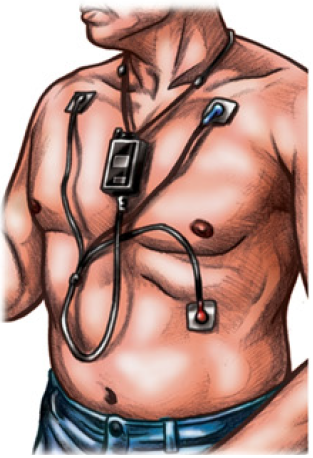
\includegraphics[width=1in]{monitor_externo_uso}
%	% where an .eps filename suffix will be assumed under latex, 
%	% and a .pdf suffix will be assumed for pdflatex; or what has been declared
%	% via \DeclareGraphicsExtensions.
%	\caption{Uso de monitor externo de eventos, tomado de  \cite{monitorizacion_ambulatoria}}.
%	\label{monitor_externo_uso}
%\end{figure}

%Pese a la mayor capacidad de diagnóstico de los monitores externos de eventos, su uso no resulta tan común como las demás tecnologías \cite{utilidad_monitor_externo}, en gran parte por los altos costos de estos equipos \cite{monitorizacion_ambulatoria} \cite{comparacion_holter_monitor} que  requieren gran capacidad para la  detección automática de la arritmia con tiempos de respuesta cortos \cite{artificial_intelligence} y disponibilidad de gran cantidad de memoria para el almacenamiento de datos \cite{journal_afib}. %Altos costos que resultan de la dificultad en la implementacion de complejos algoritmos para la detección automática de la arritmia, y en razon a que su desempeño es inversamente proporcional al tiempo de respuesta  \cite{artificial_intelligence}. 
%Al respecto del tiempo de respuesta, sobre todo en pacientes con posible toxicidad de fármacos antiarritmicos se requiere el acceso inmediato a los datos \cite{monitorizacion_ambulatoria} . Adicionalmente, en \cite{monitores_externos} y \cite{monitor_cardiaco_fibrilacion_auricular} se recalca que entre algunos parámetros importantes a obtener de la monitorización, está la duración precisa de la fibrilación  y la densidad de las arritmias en un periodo de tiempo .


%\citeauthor{embedded_arm_afib} \cite{embedded_arm_afib} resalta que diferentes herramientas computacionales para la detección de fibrilación auricular 
%varios algoritmos de reconocimiento de patrones y extracción de características 
%pueden estar limitadas en su ejecución en computadores de escritorio, en la medida que su implementación en plataformas portátiles o móviles pueden no presentar resultados satisfactorios en el tiempo de ejecución, de ahí que no se cuente con numerosas investigaciones dedicadas al estudio de posibles soluciones para la detección de fibrilación auricular en sistemas embebidos. Para el reconocimiento automático de fibrilación atrial en sistemas embebidos, se requieren mayores prestaciones en hardware en la medida de la demanda de alta exactitud y tiempos de ejecución cortos. Por un lado se requiere un alto grado de certeza en el la detección de la fibrilación auricular, y por otro, se requiere una velocidad de procesamiento adecuada. 

%Por otra parte, un computador de placa reducida, por tratarse de computador en una sola placa y de tamaño reducido,  puede utilizarse para la implementación de sistemas embebidos portables como en el caso de un Monitor Externo de Eventos Automático, y los recursos con los que actualmente se fabrican, hacen suponer un adecuado desempeño de los diferentes algoritmos mencionados para la detección automática de la arritmia tanto en su capacidad de reconocimiento como en su tiempo de respuesta, variables esenciales en la propuesta de un equipo biomédico práctico \cite{embedded_rpi}.  

%Entre los modelos supervisados más utilizados en el reconocimiento automático de fibrilación auricular se encuentran:  k vecinos más cercanos (KNN), redes neuronales artificiales (ANN), y máquinas de soporte vectorial (SVM) \cite{artificial_intelligence}. Algoritmos que en la presente investigación se implementan en un computador de placa reducida para realizar su evaluación en cuanto a capacidad de detección de fibrilación auricular y tiempo de respuesta.

Las secciones que a continuación se presentan se encuentran organizadas de la siguiente manera: en la sección 2 se realiza una descripción de la ; en la sección 3 se presenta la descripción de las ; en la sección 4 se presenta la evaluación realizada ; para último, en la sección 5 presentan las conclusiones más relevantes del estudio realizado.









\section{Materiales}

D

MAX30102
OLED
ESP32
Servidor
PC

%Para la evaluación de desempeño de los algoritmos de reconocimiento automático de patrones en la detección de fibrilación auricular en computador de placa reducida se propone el uso de la base de datos MIT-BIH AFIB (encontrada en \cite{physiobank}). Base de datos de uso generalizado en investigaciones afines y que contiene 23 registros de electrocardiografía de pacientes que presentan fibrilación auricular, con una frecuencia de muestreo de 250Hz, a una resolución de 12 bits y un rango de $+/-10mv$. Cada registro tiene una duración de 10 horas, en total se incluyen 291 episodios de fibrilación auricular con un tiempo promedio de 115 segundos, y 344 episodios de otros ritmos cardíacos \cite{wavelet_svm_afib}. Estos episodios se encuentran marcados, con anotaciones en tiempos específicos según revisiones previas de especialistas creadores de la base de datos; en la figura \ref{imagen_ecg} se representa un ejemplo de un archivo de la base de datos con la anotación respectiva en la medida que la señal cardíaca cambia llegando el segundo 5 de ritmo normal a ritmo con fibrilación auricular.

%\begin{figure}[!h]
%	\centering
%	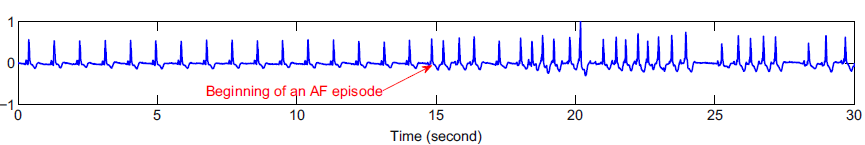
\includegraphics[width=3.5in]{base_datos_archivo.png}
%	\caption{Ejemplo de lectura de señal filtrada en archivo 4048 MIT-BIH AFIB con su anotación respectiva, tomado de \cite{wavelet_svm_afib}
%	}.
%	\label{base_datos_archivo}
%\end{figure}


%El sistema a utilizar consta de un computador de placa reducida Raspberry Pi 2 (que cuenta con un procesador quad-core ARM Cortex-A7, 1 GB de memoria RAM y puertos digitales para comunicación con diferentes periféricos \cite{rpi2}). En él se realiza el preprocesamiento, la extracción de características y el reconocimiento automático de fibrilación auricular de señales tanto guardadas en memoria como provenientes del módulo análogo digital externo ADS1115 (conversor con resolución de 16 bits y frecuencia de muestreo de 860Hz) conectado vía I2C y que permite adquirir la señal a analizar preveniente de un generador de señales. Una vez los algoritmos son ejecutados, la información es almacenada en memoria y es presentada en una pantalla TouchScreen referencia ADAFR-2097 para visualizar tanto la señal analizada como el resultado de su análisis. En la figura \ref{hardware} se representa el hardware implementado.



\begin{figure}[!h]
	\centering
	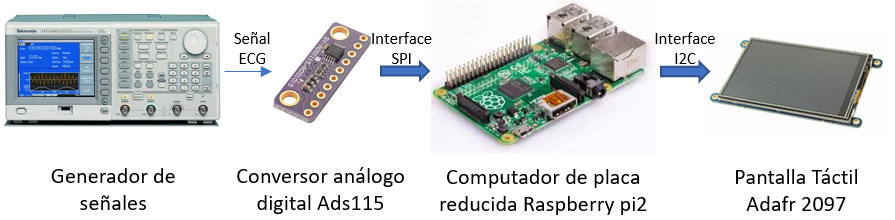
\includegraphics[width=3.5in]{hardware_partes.png}
	\caption{Esquma general de solución propuesta}.
	\label{hardware}
\end{figure}


\section{Métodos}


Estructura general del proytecto

\begin{figure}[!h]
	\centering
	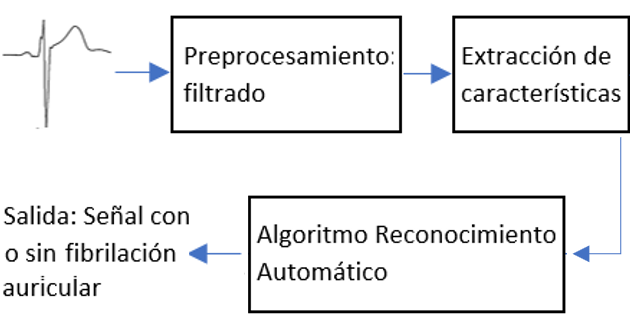
\includegraphics[width=2.5in]{estructura_general}
	\caption{Estructura general de sistema de reconocimiento de fibrilación auricular}.
	\label{estructura_general}
\end{figure}

E 

\subsection{Embebido}
Descripción de firmware 

\begin{figure*}[!t]
	\centering
	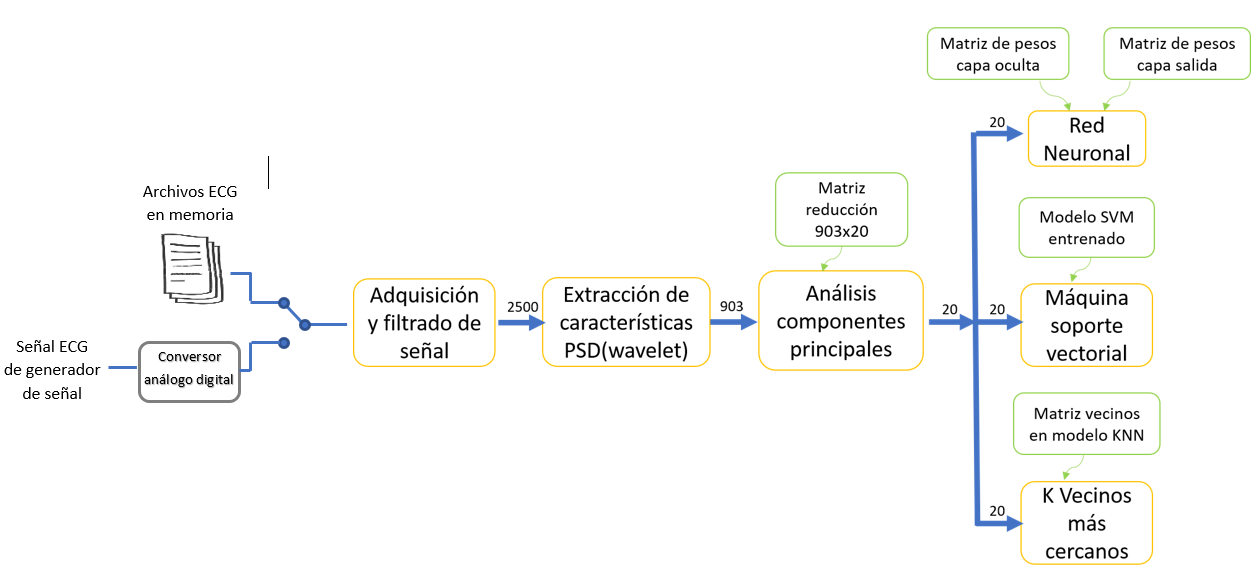
\includegraphics[width=6.5in]{diagrama_bloques_adc}%
	
	\hfil
	
	\caption{Diagrama de flujo.}.
	\label{diagrama_bloques}
\end{figure*}


\subsection{Telemetría}
Descripción de aplicacion web

%Una vez la señal de electrocardiografía es adquirida, se puede procesar computacionalmente para detectar automáticamente si presenta o no algún tipo de arritmia, en nuestro caso de estudio, fibrilación auricular (según recomendación de \cite{wavelet_svm_afib} y propuesta de  \cite{embedded_arm_afib}, la señal es procesada en ventanas de 10 segundos). Para ello, deben extraerse de la señal ciertas características que permitan distinguir fácilmente y con el mayor nivel de generalización posible, la presencia o no de la arritmia. Una vez establecidas las características, el paso siguiente es aplicar un algoritmo de reconocimiento automático de patrones que las categorice como pertenecientes a una señal con o sin fibrilación auricular, ver figura \ref{estructura_general}. Así, los algoritmos se dividen en dos etapas fundamentales, por un lado el preprocesamiento y la extracción de características, y por otro, los algoritmos de reconocimiento automático de patrones. 





%La metodología para la implementación del sistema final para el reconocimiento automático de fibrilación auricular consistió en el trabajo previo en computador personal para realizar la lectura de la base de datos MIT-BIH AFIB anteriormente presentada, determinar las características a extraer de las señales y entrenar los algoritmos con ayuda de los paquetes de procesamiento de señales y aprendizaje automático de Matlab y Python. Como resultado, se establecen concretamente las funciones matemáticas para la extracción de características y las matrices o modelos entrenados que configuran los diferentes algoritmos de reconocimiento automático a implementar en el computador de placa reducida. 


%Tanto las funciones para extraer las características de la señal de ECG a leer en el sistema propuesto, como la lectura de las matrices o modelos entrenados de los algoritmos son implementadas en el computador de placa reducida para así evaluar su desempeño en cuanto a capacidad de detección de fibrilación auricular y tiempo de respuestas asociado.



%En la figura \ref{diagrama_bloques} se presentan las diferentes etapas que componen el sistema de reconocimiento automático de fibrilación auricular propuesto, éstas se describen con mayor detalle en las siguientes subsecciones.

%\begin{figure*}[!t]
%\centering
%\subfloat[Case I]{\includegraphics[width=2.5in]{box}%
%\label{fig_first_case}}
%\hfil
%\subfloat[Case II]{\includegraphics[width=2.5in]{box}%
%\label{fig_second_case}}
%\caption{Simulation results for the network.}
%\label{fig_sim}
%\end{figure*}










%Como primera etapa, realizando la lectura de la figura \ref{diagrama_bloques} de izquierda a derecha, la señal de electrocardiografía es adquirida por dos posibles canales, uno segun la lectura de señales en archivos guardados en memoria y otro segun la adquiisición de la señal entregada por un generador de señales. La lectura de los ficheros guardados en memoria permite analizar las 28580 señales de validación para realizar la estimación estadistica de la capacidad de detección del sistema propuesto ( sensibilidad y especificidad), mientras que la adquisición de la señal entregada por el generador de señales permite la la estimación de tiempo de respuesta.


%En cuanto al preprocesamiento, con el fin de eliminar ruidos en la se señal electrocardiográfica, entre los que se encuentran: ruidos de contacto de electrodos, artefactos musculares, interferencia de línea, variaciones en línea de base, ruidos asociados al dispositivo de captura, entre otros \cite{caracterizacion_ecg}, el sistema filtra señales que presentan frecuencias inferiores a los 0.05Hz y superiores a los 40Hz. Lo anterior como se plantea en  \cite{embedded_arm_afib}, teniendo en cuenta que de hecho la actividad atrial usualmente ocurre entre las frecuencias de 4 a 9Hz. \cite{wavelet_svm_afib}


%\subsection{Extracción de características}


%En cuanto a los métodos lineales de extracción de características, las estrategias más utilizadas tratan de analizar los intervalos RR de la señal ECG (picos más altos en el trazado según l figura \ref{imagen_ecg}) \cite{comparacion_caracteristicas_afib}, información útil por ejemplo resulta ser el promedio de la duración de estos intervalos y su desviación estándar \cite{comparacion_caracteristicas_afib}. Adicionalmente, dado que la fibrilación auricular se presenta con variaciones en la onda P, también existen algoritmos que incluyen la detección  y análisis esta onda \cite{temp_svm_afib}. De hecho, es común encontrar dispositivos comerciales que realizan este tipo de extracción de características \cite{new_englad_journal} \cite{journal_afib}

%El análisis temporal de la señal de electrocardiografía presenta sin embargo un mayor reto para la adecuada detección de fibrilación auricular por la obligada detección eficaz de las ondas R y P, dado que por ejemplo las ondas P son muy propensas a contaminación con señales de  movimientos y artefactos, y de hecho, su no detección degrada por completo la detección de la arritmia \cite{artificial_intelligence}. Aquí hay un esfuerzo mayor por depurar el algoritmo de detección de picos que a su vez son propensos a ruido y errores de procesamiento \cite{wavelet_svm_afib}


%Por otro lado, la caracterización en frecuencia de la señal ECG también es una alternativa útil, aquí se incluye el análisis de Fourier y el cálculo de la densidad espectral de potencia. Si bien este método cuenta con una buena resolución frecuencial, la incertidumbre en la localización temporal de la energía resulta ser su principal desventaja \cite{caracterizacion_ecg}. 


%Por último, para suplir la falta de ubicación temporal de las energías discriminadas frecuencialmente, se plantean las representaciones tiempo-frecuencia, permitiendo, según una resolución deseada, mediar entre la incertidumbre de frecuencia y la de la ubicación exacta. Al respecto, la transformada Wavelet discreta ha tomado mayor popularidad en cuanto a que permite la descomposición en niveles de escala diferentes (el inverso de la frecuencia) de la señal, a lo largo del tiempo \cite{comparacion_caracteristicas_afib}. Esta transformada representa una señal en una secuencia de coeficientes basados en bases ortogonales $\psi$ de ondas finitas (wavelet madre, trasladada ($\tau$) y escalada en el tiempo($s$)). Como en la ecuación \ref{wavelet_ecuation}, se define la transformada wavelet para señales discretas como la correlación entre la señal y la función $\psi$ escalada y trasladada en el tiempo \cite{clasificacion_pvc_no_supervizado}.

%\begin{equation}\label{wavelet_ecuation}
%[W_\psi f](s,\tau)= A\sum\sum_{}^{} \psi_{s,\tau} \left(s,\tau \right)f(t)
%\end{equation}



%\subsubsection{Implementación  extracción de características}

%Con base en las investigaciones de \cite{wavelet_svm_afib}, se estudió como estrategia de extracción de características, la implementación de los algoritmos de Transformada Wavelet Estacionaria hasta el nivel 7 y sobre cada una de las sub bandas, el cálculo de la densidad espectral de potencia. Esta información, que incluye 903 datos por cada señal analizada(como lo representa la figura \ref{diagrama_bloques}) debe ingresarse a un algoritmo de análisis de componentes principales que permita disminuir la cantidad de datos y por ende el fácil entrenamiento y uso de los algoritmos siguientes de reconocimiento automático de patrones. Como lo representa la misma figura, en trabajos preliminares en computador personal, se determina la matriz de reducción de características que es leída como un archivo .csv por el computador de placa reducida para así disminuir el número de variables a 20. 

%Hasta aquí, en el computador de placa reducida se implementan las funciones que permiten el filtrado adecuado de la señal y la extracción de características (densidad espectral de potencia de las 7 sub bandas según descomposición wavelet); para por último, mediante el uso de la matriz de reducción de características previamente guardada en la memoria, disminuir el número de características que ingresan a los diferentes algoritmos de reconocimiento automático de patrones que van a ser evaluados según su previo entrenamiento. Las funciones de filtrado, extracción de características y reducción de dimensión se logran haciendo uso de las librerías \textit{numpy} y \textit{scipy} de Python.



%\subsection{Algoritmos de reconocimiento automático de patrones}


%Una vez extraídas las características, es posible aplicar un algoritmo de reconocimiento automático de patrones que previamente entrenado sepa distinguir entre características procedentes de una señal con o sin fibrilación auricular.

%En general, los algoritmos de reconocimiento automático de patrones utilizan en primera instancia un conjunto de datos para su entrenamiento y otro para su validación, ambos provenientes generalmente de bases de datos con alto grado de aceptación científica.  De la lectura de los 23 archivos de 10 horas cada uno de la base de datos MIT-BIH AFIB, y considerando las observaciones adicionales que acompañan la colección de los archivos en relación con la ausencia de algunos paquetes de datos, se extrajeron 33625 señales, cada una relacionado con la lectura de 10 segundos de información (2500 muestras). Este conjunto de datos se dividió aleatoriamente en dos subconjuntos: uno representando al 85\% de la base de datos para el entrenamiento de los algoritmos, y el otro al 15\% restante para la validación y caracterización de desempeño de los algoritmos.

%El conjunto de entrenamiento resultante está compuesto por 19317 señales sin fibrilación auricular y 9263  señales con fibrilación auricular; mientras que para el caso del conjunto de validación se cuenta con 3410  señales con fibrilación auricular y 1635 muestras catalogadas como sin fibrilación auricular.  En la figura \ref{division_BD}  se ilustra la partición de la base de datos.



%\begin{figure}[!h]
%	\centering
%	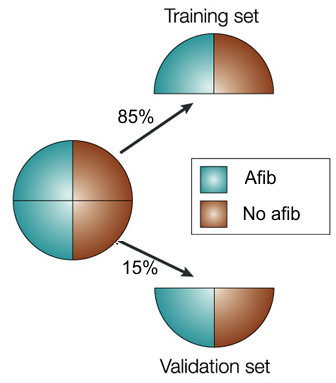
\includegraphics[width=1.5in]{conjunto_validacion_entrenamiento.png}
%	\caption{División de base de datos en conjuntos de entrenamiento y validación, editado de \cite{train_validation_set}}.
%	\label{division_BD}
%\end{figure}


%Con el conjunto de datos de entrenamiento, es posible caracterizar el algoritmo de reconocimiento de patrones que maximice la discriminación entre las categorías a clasificar. Y una vez entrenado, conviene especificar las medidas de su desempeño estadístico en cuanto a su respuesta para la clasificación de nuevas señales (datos del conjunto de validación). Aquí es importante recalcar que este conjunto de datos no ha sido usado en ninguna medida en el proceso de entrenamiento, e incluye su categorización clara según criterio científico, en nuestro caso el concepto médico.  Este conjunto incluye $P$ muestras con fibrilación auricular (muestras positivos) y $N$ muestras sin ella (muestras negativas). 

%Entre los parámetros más usados para caracterizar el desempeño se encuentran la sensibilidad, y especificidad. Si el algoritmo clasificador clasifica adecuadamente $TP$ fibrilaciones auriculares (Verdaderos positivos), la sensibilidad puede expresarse como en la ecuación \ref{ecuacion_sensibilidad}, siendo $FN$ el número de falsos negativos. Por otro lado, si se clasifican adecuadamente $TN$ señales sin fibrilación auricular (verdaderos negativos), la especificidad puede expresarse como en la ecuación \ref{ecuacion_especificidad}, siendo  $TN$ el número de verdaderos negativos. %Por ultimo, la precisión se calcula como lo referencia la ecuación \ref{ecuacion_precisión}.



%\begin{equation}
%TPR=\frac{TP}{TP+FN}
%\label{ecuacion_sensibilidad}
%\end{equation}
%
%\begin{equation}
%TNR=\frac{TN}{FP+TN}
%\label{ecuacion_especificidad}
%\end{equation}



%Por otra parte, en cuanto a la velocidad o  tiempo de respuesta del sistema en la detección de fibrilación auricular, es usual medir el tiempo de predicción del algoritmo  \cite{clasificacion_pvc_no_supervizado}, estimado como  el tiempo de transición (tiempo de espera para detección de cambios de señal con o sin fibrilación atrial)\cite{wavelet_svm_afib}.


%En resumen, sensibilidad  hace relación a la medición de la proporción de positivos (en nuestro caso, señales con fibrilación auricular) correctamente identificados;  especificidad mide la proporción de negativos (señales sin fibrilación auricular) que son correctamente identificados como tal; y tiempo de respuesta hace referencia al tiempo que tarda un algoritmo determinado en detectar una transición a fibrilación auricular.







%\subsubsection{Redes neuronales}
%Su uso computacional pretende modelar el comportamiento del cerebro biológico mediante la interconexión de muchas neuronas para procesar información de entrada (características) y generar una salida (decisión si las características corresponden o no fibrilación auricular). 


%Cada una de las neuronas corresponden a los puntos de unión donde se realizan las sumas de la multiplicación de cada entrada por un peso previamente establecido, el esquema se repite con nuevas capas aumentando la complejidad del algoritmo clasificador. En este caso, previamente la red neuronal es entrenada para establecer el valor de cada uno de los pesos, el entrenamiento se hace ajustando iterativamente los pesos según la lectura de bases de datos en los que se conoce a priori la presencia o no de la arritmia.





%\begin{figure}[!h]
%	\centering
%	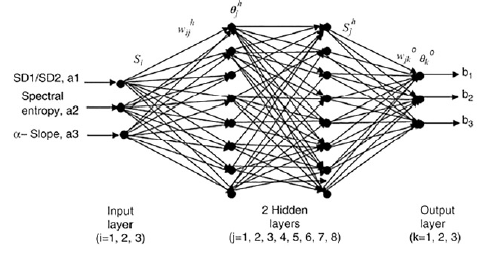
\includegraphics[width=3in]{red_neuronal}
%	\caption{Red neuronal artificial, tomado de  \cite{artificial_intelligence}}.
%	\label{red_neuronal}
%\end{figure}


%Para el caso de la red neuronal artificial a implementar en el computador de placa reducida, dadas las recomendaciones de \cite{comparacion_caracteristicas_afib} y \cite{handheld_arm_cardiac_event_monitor} en el entrenamiento con coeficientes wavelet como caracaterísticas para el reconocimiento de fibrilación auricular, se escoge como topología una red neuronal feed-forward perceptrón con tres capas con función de activación sigmoidal; su función de transferencia se presenta en la ecuación \ref{eqn_redneuronal} con $x$ el vector de características a analizar, $IW$ y $b1$ los pesos de la capa oculta,   y $LW$ con $b2$ los pesos de la capa de salida.

%Sobre esta topología según los mismos autores, se procede a variar el número de neuronas en la capa oculta para estimar la configuración que maximice la capacidad de respuesta del modelo; para cada una de las configuraciones se realiza la validación cruzada del modelo según la lectura de las muestras en el conjunto de entrenamiento. Como resultado de la mejor configuración,  Se implementó finalmente una red con 10 neuronas en la capa oculta y una neuronal en la capa de salida

%\begin{equation}
%\label{eqn_redneuronal}
%f(x)=sigmod(LW*sigmod((IW*x)+b1)+b2)
%\end{equation}


%\textcolor{black}{Las matrices que contienen los pesos de las diferentes neuronas $LW$, $IW$, $b1$ y $b2$, son guardadas en archivos .csv con una precisión de 9 cifras decimales para su almacenamiento en la memoria del computador de placa reducida y su lectura al momento de ejecutar la red neuronal. Los archivos generados ocupan 4 kbytes en memoria.}




%\subsubsection{Máquinas de soporte vectorial}

%Partiendo de un conjunto de muestras (en el espacio de características) con o sin fibrilación auricular, éste modelo busca un hiperplano que separe todas las muestras en dos subespacios, de tal modo que al tener un nuevo dato (vector características), es posible determinar de qué lado de la separación se encuentra, y así establecer si corresponde al subespacio con fibrilación auricular o sin ella. Adicionalmente, SVM procura establecer el mayor nivel de margen entre las dos categorías a clasificar, la inclusión adicional de kérneles permite implementar hiperplanos de separacion de mayor complejidad.   %como se muestra en la figura \ref{svm} \cite{wavelet_svm_ann_afib}. 

%En la ecuación \ref{svm_ecuation} se presenta su función de clasificación, siendo $x$ el vector de características a clasificar;  $k$ la función kernel, $b$ el margen de separación, $\alpha_{i}$ los coeficientes de lagrange y $x_{i}$ el iésimo vector de soporte,  estos parámetros resultantes del proceso de entrenamiento.
%\begin{figure}[!h]
%	\centering
%	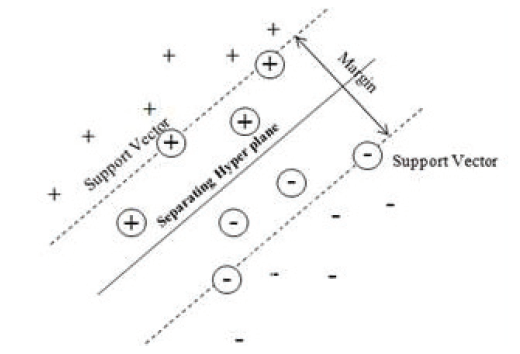
\includegraphics[width=2.8in]{svm}
%
%	\caption{Máquina de soporte vectorial, tomado de  \cite{arrhythmia_astronauts}}.
%	\label{svm}
%\end{figure}
%
%\begin{equation}\label{svm_ecuation}
%f(x)= \sum_{i=1}^{n}\alpha_{i}(k(x,x_{i})+b) %\psi_{s,\tau} \left(s,\tau \right)f(t)
%\end{equation}

%\begin{equation}
%\label{eqn_svm}
%1
%%\sum_{i=1}^{n}%\alpha_{i}
%
%\end{equation}

%En la figura \ref{svm}, se trata del caso simple bidimensional, donde se han analizado todas las muestras para determinar el hiperplano de separación óptimo. El algoritmo se puede aplicar también para el caso n dimensional, con la posible inclusión adicional de kérneles para subespacios separables a un nivel de complejidad mayor.

%Para la implementación de la máquina de soporte vectorial, según la revisión de \cite{wavelet_svm_afib}, quien utiliza como características la densidad espectral de potencia de los coeficientes wavelet, se parte de un kernel gausiano con valores $\gamma=0.01$ y $C=100$. Y sobre estos valores iniciales, se procede a realizar pruebas con distintos valores de $\gamma$ y $C$ (como lo sugieren \cite{comparacion_caracteristicas_afib}). Los modelos son entrenados en el lenguaje de programación de Python con ayuda de la librería Scikit-learn. Como resultado, se escogieron los parámetros $\gamma=10$ y $C=1$ en la configuración de la máquina de soporte vectorial con kernel gausiano, dado que presentó mejores resultados. Como se trata aquí de exportar el modelo al computador de placa reducida, conviene serializar el objeto y así poder leerlo con el mismo paquete de librerías con el que se entrenó. Al serializar el objeto, con la ayuda del paquete \textit{pickle}, éste se convierte en  una cadena de bytes de bajo tamaño y rápida lectura. El fichero resultante del modelo entrenado de la máquina de soporte vectorial  corresponde a un archivo con extensión .pkl de 0.9 Mbytes, el fichero incluye los vectores soporte, el tipo de kernel utilizado y los parámetros correspondientes.
%
%
%
%
%
%\subsubsection{K vecinos más cercanos}
%
%Este clasificador, a diferencia de los anteriores, no requiere etapa  de entrenamiento \cite{hybrid_classifier}, y está basado en el análisis de la distancia geométrica entre una nueva muestra y las demás del conjunto de entrenamiento. Para ilustrar con un ejemplo, como se presenta en la figura \ref{wiki:knn}, un nuevo vector de características es clasificado en una de las categorías,  si al revisar geométricamente un número determinado de vecinos, este se encuentra en una vecindad mayoritaria de determinada categoría. Así, el algoritmo incluye el cálculo de las distancias y el conteo de vecinos más cercanos de cada categoría.
%
%
%\begin{figure}[!h]
%	\centering
%	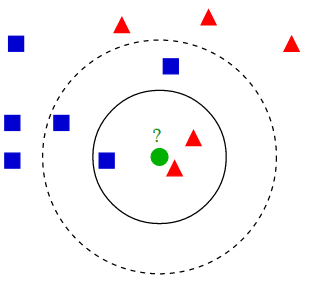
\includegraphics[width=1.82in]{knn}
%
%	\caption{K vecinos más cercanos, tomado de  \cite{wiki:knn}, la nueva muestra (verde) se clasifica como roja.}.
%	\label{wiki:knn}
%\end{figure}
%
%Por último, haciendo nuevamente uso de la liberia \textit{Scikit-learn} de \textit{python}, el clasificador de K vecinos más cercanos propuesto utiliza la distancia Euclidiana como medida de similaridad \cite{comparacion_caracteristicas_afib}.
%Como se plantea en \cite{comparacion_caracteristicas_afib} se procede a variar el número de vecinos en el modelo y comparar su precisión mediante validación cruzada. Como resultado, se escogió el valor $k=10$ como parámetro y una vez entrenado el modelo se procede a serializar el objeto el archivo después de la serialización tiene un tamaño de 9.6 Mb, valor superior al del tamaño de la máquina de soporte vectorial y la red neuronal en la medida dado que aquí el archivo relaciona todos los vecinos, es decir muestras en el espacio de características, teniéndose en este caso un vector por cada muestra del conjunto de entrenamiento de la base de datos.
%
%El computador de placa reducida lee los archivos .csv con las matrices y los serializados en formato .pkl  para configurar los objetos de clasificación de fibrilación auricular previa extracción de características, como se ilustra en la figura \ref{diagrama_bloques}. Y una vez implementado el sistema, es posible realizar la lectura de las señales del conjunto de datos de validación para así caracterizar el desempeño de cada algoritmo.
%
%
%
%%\subsubsection{Clasificador Híbrido}
%%
%%Como se ha presentado anteriormente, diferentes algoritmos presentan desempeños diferentes en la detección de arritmias, y es este mismo hecho el que posibilita la creación de clasificadores adicionales con base en la integración de clasificadores individuales. Esta integración se conoce como clasificadores Híbridos.
%%
%%Para obtener mejores resultados con la implementación de clasificadores híbridos, se requiere que los diferentes clasificadores tengan errores de clasificación diferentes, situación fácilmente predecible en razón a que ANN, KNN Y SVM son teórica y estructuralmente diferentes \cite{hybrid_classifier}. \cite{hybrid_classifier} y \cite{hybrid_engine} obtuvieron una mejora en la clasificación de arritmias cardíacas utilizando clasificadores híbridos en comparación con el desempeño de clasificadores individuales.
%%
%%Entre las técnicas para la implementación de clasificadores híbridos se encuentran: voto mayoritario, bagging , dagging y DECCORATE. \cite{hybrid_astronauts} encontraron que en detección de arritmias el ensamble que mejores resultados presenta es el de voto mayoritario. Tratándose éste de un arreglo de clasificadores independientes en el cual se examina la respuesta de cada uno de ellos como si se tratase de un conteo de votos, y dependiendo la salida que haya obtenido mayor numero de votos, esta se reflejará en la salida.
%%
%%
%%
%
%
%
%
%
%
%
%
%
%
%
%
%

\section{Resultados}

%%Con la implementación de los elementos presentados en la figura \ref{hardware} y con las herramientas de la figura \ref{diagrama_bloques}, 
%En la figura \ref{montaje_generador_rpi} se presenta el montaje final para la evaluación de desempeño de los diferentes algoritmos de reconocimiento automático de fibrilación auricular. El computador de placa reducida permite la lectura tanto de ficheros guardados en memoria para la determinación de sensibilidad y especificidad, como de la señal análoga proveniente del generador de señales para la estimación de tiempo de respuesta en la detección de fibrilación auricular.

\begin{figure}[!h]
	\centering
	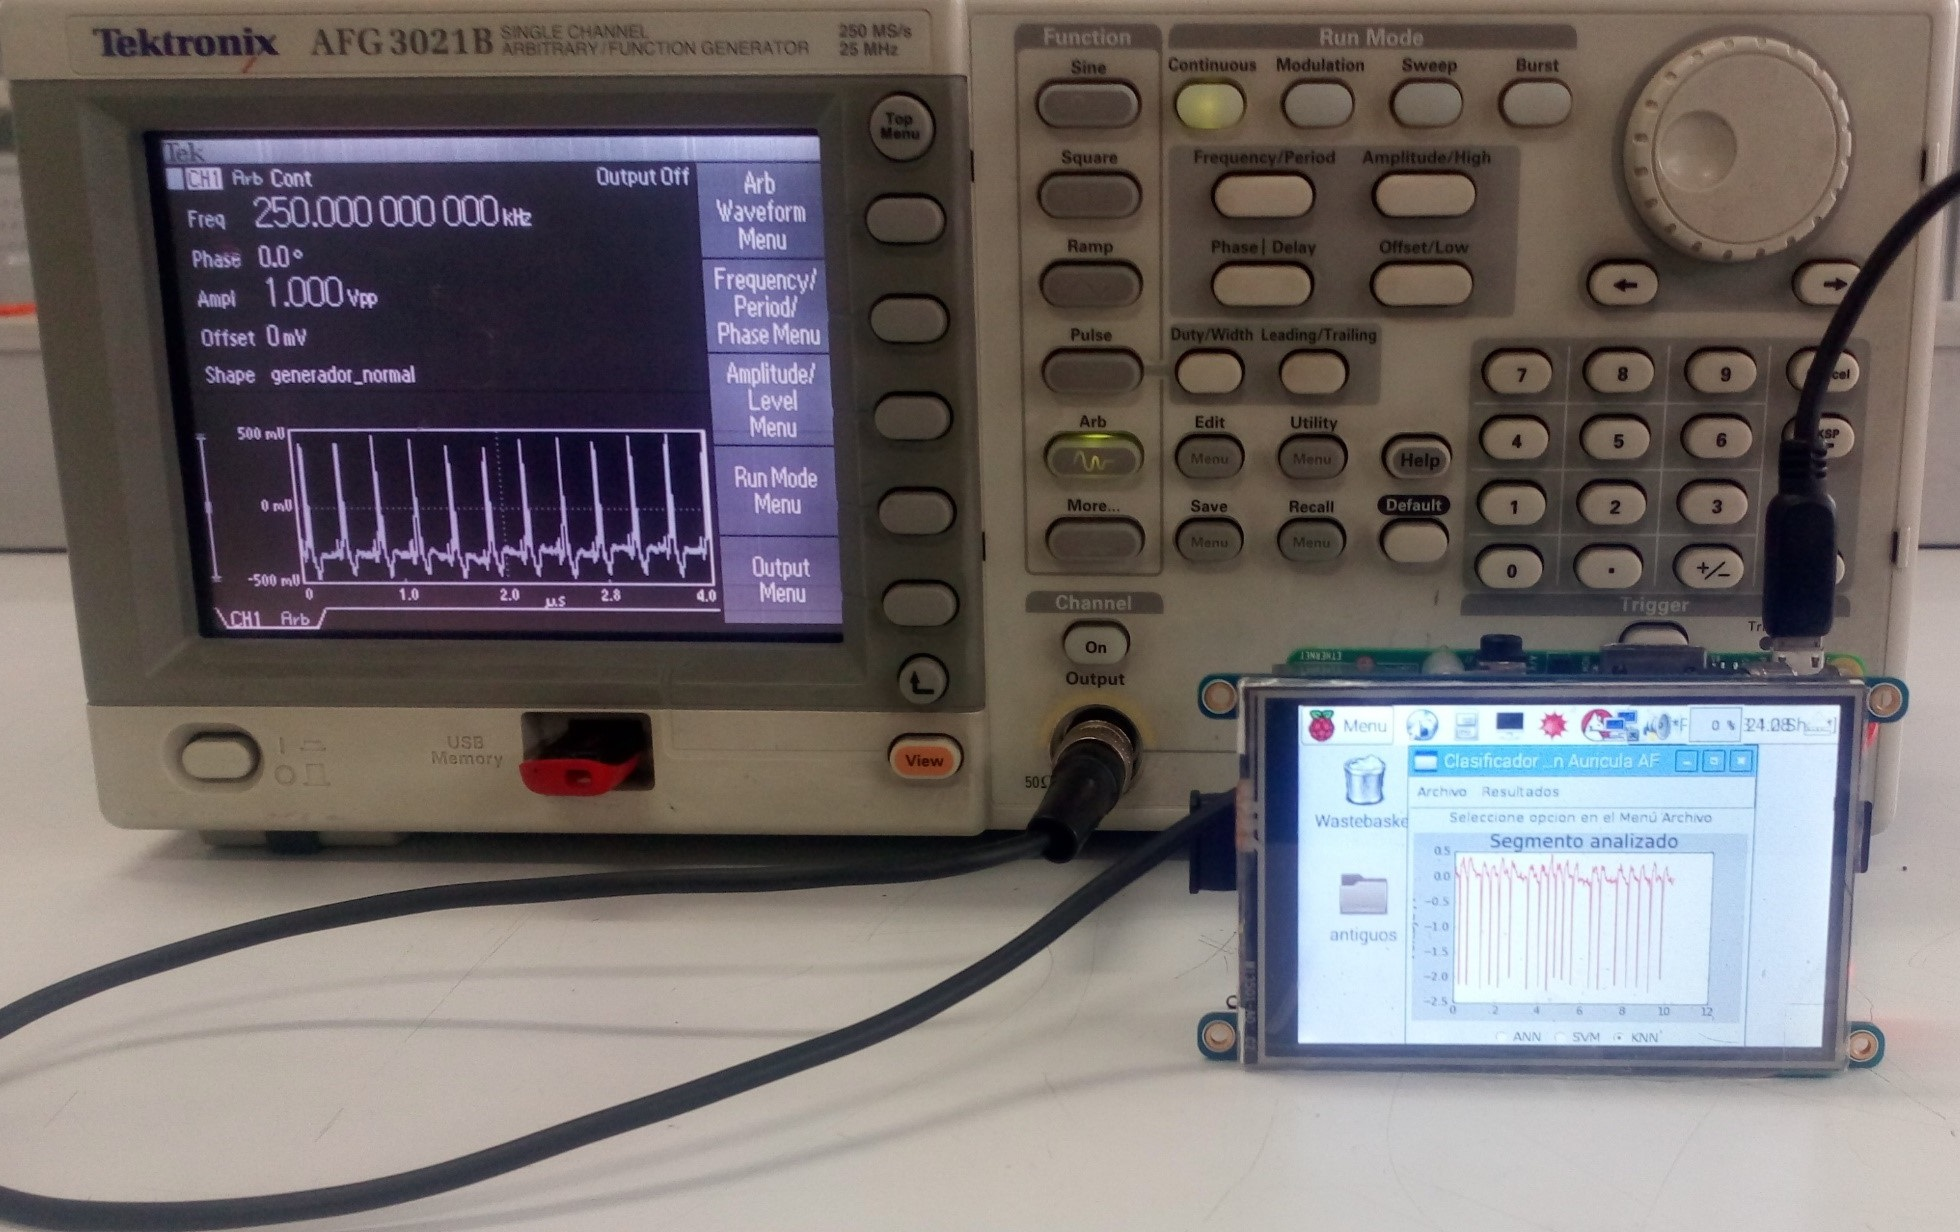
\includegraphics[width=2.5in]{montaje}
	% where an .eps filename suffix will be assumed under latex, 
	% and a .pdf suffix will be assumed for pdflatex; or what has been declared
	% via \DeclareGraphicsExtensions.
	\caption{Montaje .}
	\label{montaje_generador_rpi}
\end{figure}


\begin{figure}[!h]
	\centering
	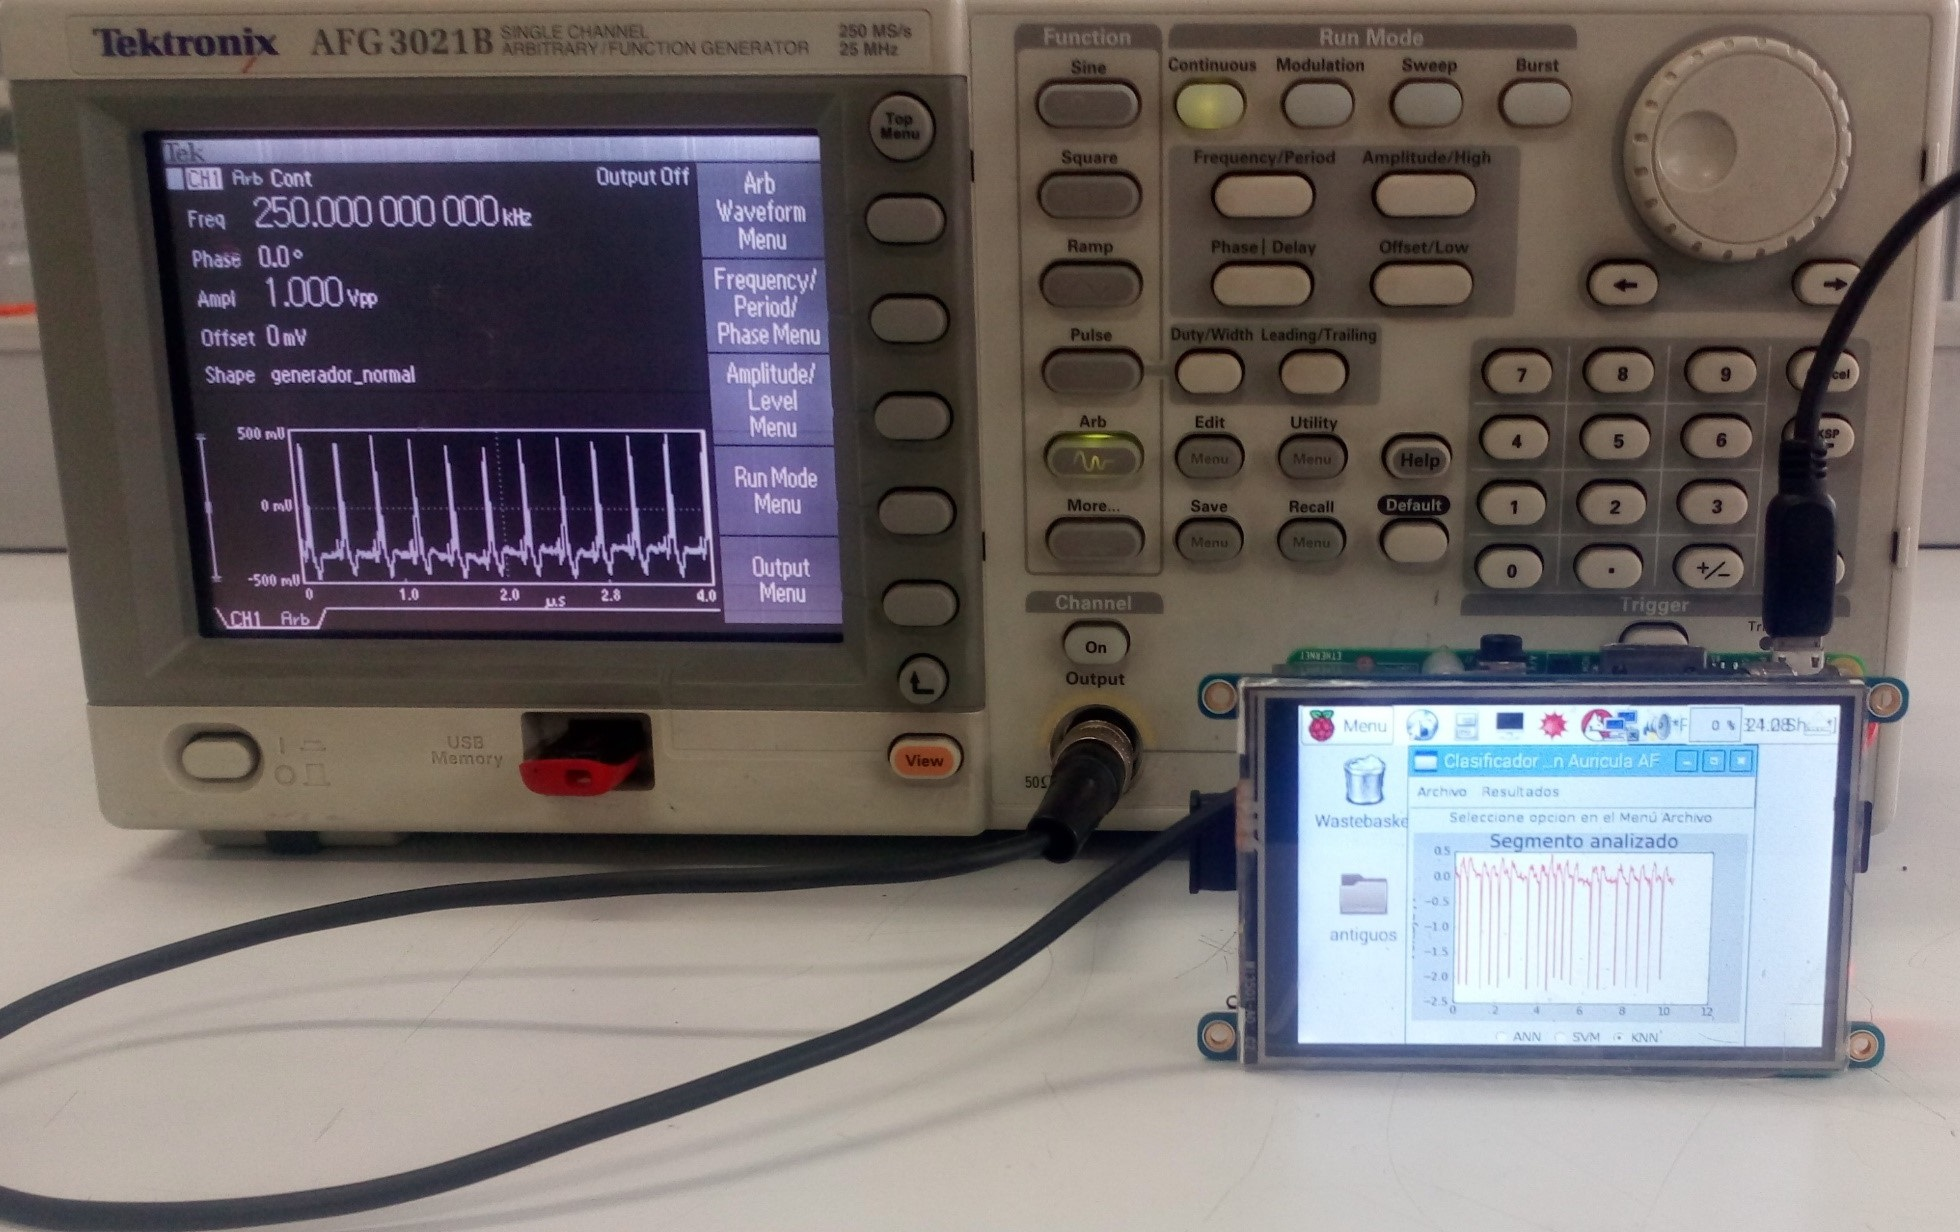
\includegraphics[width=2.5in]{montaje}
	% where an .eps filename suffix will be assumed under latex, 
	% and a .pdf suffix will be assumed for pdflatex; or what has been declared
	% via \DeclareGraphicsExtensions.
	\caption{Montaje para la obtención de resultados, simulador.}
	\label{montaje_generador_rpi}
\end{figure}

\begin{figure}[!h]
	\centering
	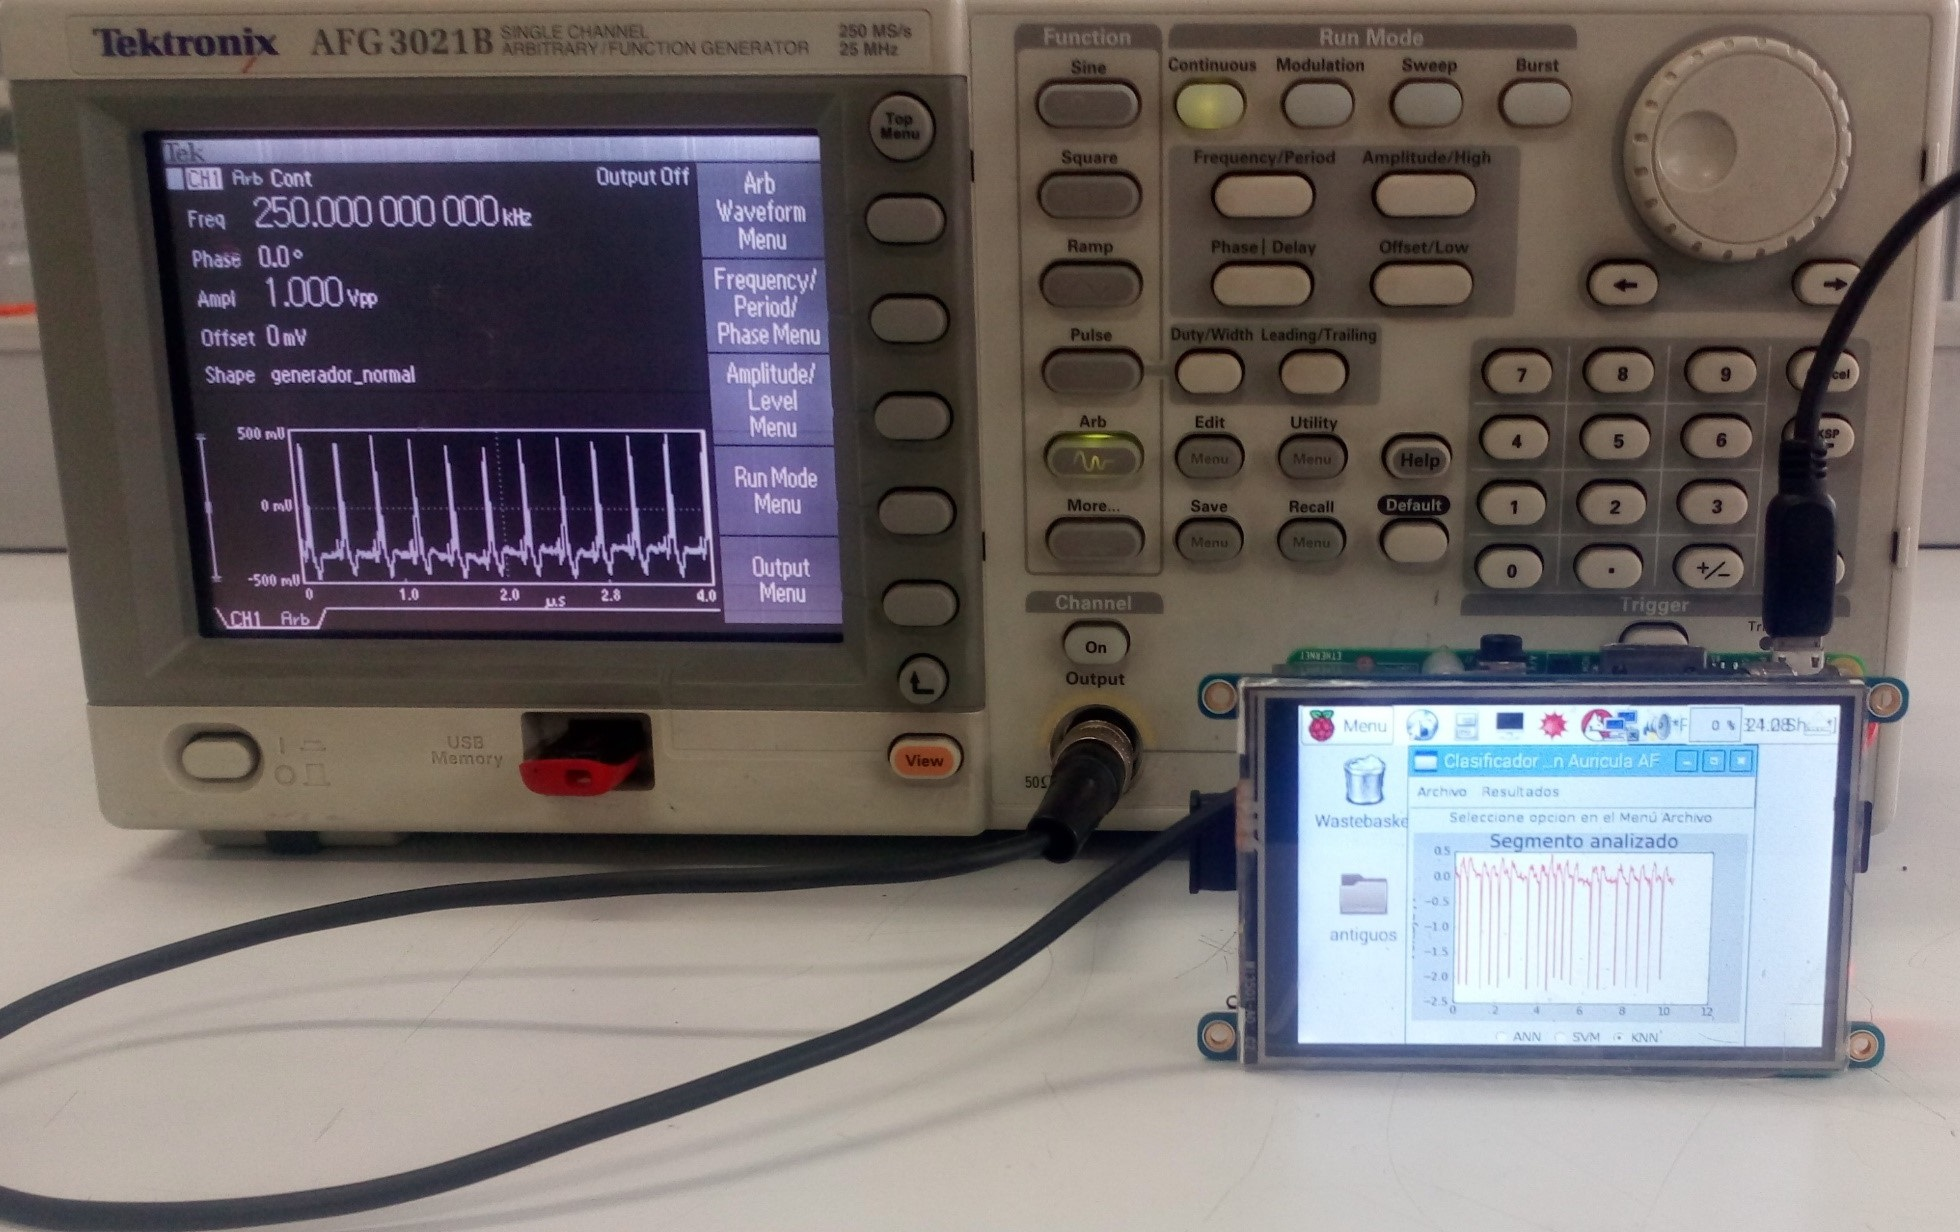
\includegraphics[width=2.5in]{montaje}
	% where an .eps filename suffix will be assumed under latex, 
	% and a .pdf suffix will be assumed for pdflatex; or what has been declared
	% via \DeclareGraphicsExtensions.
	\caption{Aplicacion web.}
	\label{montaje_generador_rpi}
\end{figure}

%
%\textcolor{black}{En cuanto a la capacidad para detectar las señales con o sin fibrilación auricular}, se utilizan las ecuaciones de sensibilidad y especificidad \ref{ecuacion_sensibilidad} y \ref{ecuacion_especificidad}. Estimativos según la respuesta del sistema propuesto dado el análisis de cada una de las 5045 señales de validación, \textcolor{black} {esta vez}  guardadas en memoria. Una vez realizada la lectura de todas las señales de validación, se contabilizaron para cada uno de los algoritmos (ANN, KNN y SVM) el número de verdaderos positivos, verdaderos negativos, falsos positivos y falsos negativos. En el cuadro \ref{cuadro:resultados_sn_sp} se presentan los valores de sensibilidad y especificidad para cada uno de los algoritmos planteados.


	\begin{table}[h!]
	\centering
	
	\caption{Resultados Sensibilidad y Especificidad  algoritmos implementados
	}
	%\cite{ica_bayes_gmm_afib} }
	\def\arraystretch{1.2}%  controla padding
	\begin{tabular}{c c l}
		%		\toprule
		
		\hline
		\textbf{Algoritmo} & \multicolumn{1}{c}{\textbf{Sn}} & \textbf{Sp}	\\ 
		\hline
		Red Neuronal  & 91.9\%	& 96.8\%\\
		%\hline
		Máquina de soporte vectorial  & 94.5\%	& 97.5\%\\		
		%\hline
		K vecinos más cercanos & 95.8\%	& 96.6\%\\
		
		\hline
		%\bottomrule
	\end{tabular}%
	\label{cuadro:resultados_sn_sp}%
\end{table}%




%En general el algoritmo que presentó mejor desempeño en la detección de fibrilación auricular fue el de k vecinos más cercanos, seguido por el de máquina de soporte vectorial y por último la red neuronal.  Lo anterior en cuanto a la detección tanto de señal con fibrilación auricular como de señales sin fibrilación auricular. %Resultados similares a los presentados por \cite{artificial_intelligence} quien realiza una revisión de diferentes investigaciones realizadas con estos mismos algoritmos para el reconocimiento de fibrilación auricular con variadas metodologías para la extracción de características.
%
%Los resultados encontrados son superiores a diversas investigaciones que utilizan también una ventana de trabajo corta como la utilizada en la presente investigación
%\cite{window_size_performance} \cite{pc_10latidos_intervalosRR_svm}. Aunque existen investigaciones que documentan resultados aún superiores a los presentados en el presente trabajo \cite{wavelet_svm_afib}, en ellas no se documentan específicamente el tratamiento, selección o omision de señales que se realiza con la base de datos.
%
%
%En cuanto a la revisión del tiempo de cómputo requerido para la ejecución de los diferentes algoritmos, se encontró que todos los algoritmos tardaron en el computador de placa reducida $0.7$ $s$ antes de procesar los nuevos datos que esperan a su procesamiento en tiempo real. Y de este tiempo de computo se encontró que el $95\%$ corresponde a las líneas de código destinadas a la extracción de características y el restante a la evaluación de los modelos sea ANN, SVM o KNN. Por lo que pese a que algunos modelos pueden resultar más complejos en su uso computacional (por ejemplo KNN), su uso no representa una contribución representativa  en el tiempo de computo final.

%\begin{table}[h!]
%	\centering
%	
%	\caption{Tiempos de cómputo de algoritmos implementados
%	}
%	%\cite{ica_bayes_gmm_afib} }
%	\def\arraystretch{1.2}%  controla padding
%	\begin{tabular}{c c}
%		%		\toprule
%		
%		\hline
%		\textbf{Algoritmo} & \multicolumn{1}{c}{\textbf{Tiempo de Cómputo}} \\ 
%		\hline
%		Extracción de características & 0.667 s \\
%		Red Neuronal  & 0.027 s	\\
%		%\hline
%		Máquina de soporte vectorial  & 0.037 s	\\		
%		%\hline
%		K vecinos más cercanos & 0.067 s	\\
%		
%		\hline
%		%\bottomrule
%	\end{tabular}%
%	\label{cuadro:tiempo_computo}%
%\end{table}%



%Por otra parte, para la evaluación del tiempo de respuesta de los algoritmos en computador de placa reducida para la detección en tiempo real de fibrilación auricular, se realiza la lectura de señal análoga por medio del \textcolor{black}{modulo conversor análogo digital conectado vía serial al computador de placa reducida}, la señal que ingresa al sistema es la suministrada por un generador de señales que tiene \textcolor{black}{almacenados los segmentos de fibrilación auricular precedidos por señales sin esta arritmia}. De modo que ante cada cambio de señal se calcula su tiempo de respuesta, previa sincronización de las medidas realizadas. En el cuadro \ref{cuadro:resultados_tiempo_respuesta} se presentan los resultados obtenidos para los diferentes algoritmos. En general los algoritmos detectan fibrilación auricular después de un tiempo cercano a la longitud de la ventana escogida para el entrenamiento y ejecución de la aplicación (10 s), y la varianza presenta valores elevados en la medida que los algoritmos no solo fueron entrenados con los cambios de señal sin fibrilación auricular a señales con ella, si no que por la naturaleza de la base de datos utilizada se presentó un mayor entrenamiento con intervalos no relacionados con dicha transición (hay muchas más muestras con fibrilación sostenida que paroxismal).
%
%
%\begin{table}[h!]
%	\centering
%	
%	\caption{Resultados tiempo de respuesta de algoritmos implementados
%	}
%	%\cite{ica_bayes_gmm_afib} }
%	\def\arraystretch{1.2}%  controla padding
%	\begin{tabular}{c c l}
%		%		\toprule
%		
%		\hline
%		\textbf{Algoritmo} & \multicolumn{1}{c}{\textbf{Media}} & \textbf{Varianza}	\\ 
%		\hline
%		Red Neuronal  & 7.12 s& 12.08 s\\
%		%\hline
%		Máquina de soporte vectorial  & 6.17 s	& 10.08 s\\		
%		%\hline
%		K vecinos más cercanos & 6.05 s	& 8.36 s\\
%		
%		\hline
%		%\bottomrule
%	\end{tabular}%
%	\label{cuadro:resultados_tiempo_respuesta}%
%\end{table}%





\section{Conclusiones}

%La extracción de características en el dominio tiempo frecuencia utilizada presenta buenos resultados para el desempeño de algoritmos de reconocimiento automático de fibrilación auricular. Los valores de sensibilidad, especificidad  obtenidos para los algoritmos ANN, SMV y KNN son equiparables a los de diversas investigaciones a fines en aplicaciones no embebidas con variadas metodologías para la extracción de caracterrísticas,  como se relacionan en \cite{artificial_intelligence} 
%
%Resultados similares a los presentados por \cite{artificial_intelligence} quien realiza una revisión de diferentes investigaciones realizadas con estos mismos algoritmos para el reconocimiento de fibrilación auricular con variadas metodologías para la extracción de características.
%
%La metodología utilizada en cuanto al uso de coeficientes wavelet sobre ventanas de 10 segundos, el entrenamiento y la importación de modelos entrenados de KNN, SVM y ANN es adecuada en cuanto a la detección en tiempo real de fibrilación auricular con el sistema embebido propuesto dados los tiempos de computo y de respuesta encontrados . 
%
%%En cuanto a los modelos entrenados de los algoritmos KNN SVM y ANN, si bien existen diferencias sustanciales en cuanto al tamaño de información que los representan, las capacidades computacionales de un computador de placa reducida permiten su ejecución en tiempo real adecuada segun la metodología utilizada. 
%En cuanto al tiempo de computo, si bien existen diferencias sustanciales en cuanto al tamaño de información que representan a los modelos ANN, SVM, y KNN entrenados, se requiere mucho más tiempo para la extracción de características que para la ejecución de estos modelos. Por ello, trabajar con ventanas aún más cortas que la utilizada en la presente investigación requeriría una revisión previa de la metodología utilizada para garantizar su operación en tiempo real.







\section*{Acknowledgment}
We acknowledge the acknowledged acknowledgees.

\bibliography{bibit}
\bibliographystyle{IEEEtranN}

\end{document}